\documentclass[a4paper,12pt,titlepage, twoside]{report} 

\usepackage[latin1]{inputenc}
\usepackage{amssymb}
\usepackage{amsthm}
\usepackage[fleqn]{amsmath}
\usepackage{xcolor}
\usepackage{relsize}
\usepackage{paralist}
\usepackage{graphicx}
\usepackage[linesnumbered, ruled]{algorithm2e}

\usepackage{pdfpages}



\newcommand{\suaca}{\textbf{SUACA}}
\newcommand{\microop}{$\mu$op}
\newcommand{\microops}{$\mu$ops}

%\usepackage{bnf}
%\usepackage{epsf}
\usepackage{appendix}

%\usepackage[a4paper]{geometry}
%\geometry{left=3cm,right=3cm,top=23mm,bottom=25mm,head=14.5pt}

\usepackage{phdthesis}
\setlength{\headheight}{15pt}
\usepackage{listings}
\lstset{showspaces=false,showstringspaces=false,breaklines=true,breakindent=0pt,
        prebreak={},
        postbreak=\mbox{{ }}}

\usepackage{makeidx}          % wir wollen auch einen Index
\usepackage{hyperref} 
\usepackage{tikz}
\usetikzlibrary{matrix,backgrounds, shapes, arrows.meta}
\tikzset{mynode/.style={draw, ellipse, thick, line width = 2pt}}
\usepackage{tkz-graph}
\SetUpEdge[lw         = 1.5pt,
           style={->},
           color      = black,
           labelcolor = white,
           labeltext  = red,
           labelstyle = {draw,text=black}]

\tikzset{bright/.style = {bend right=23, ->}}
\tikzset{bleft/.style = {bend left=23, ->}}


\usepackage{pgfplots}
\usepackage{changepage}
\usepackage{fancyvrb}
\parindent0pt
\newtheorem{theorem}{Theorem}
\newtheorem{definition}{Definition}

\begin{document}
\setlength{\oddsidemargin}{\dimexpr (\paperwidth-\textwidth)/2 - 1in\relax}
\setlength{\evensidemargin}{\oddsidemargin}

\begin{titlepage}
\setlength{\topmargin}{0cm}

\begin{changetext}{2cm}{0cm}{0cm}{0cm}{0cm}
   
  

%\let\footnotesize\small \let\footnoterule\relax
\begin{center}

%\hbox{}
%\vfill

\includegraphics[width=4cm]{eule}
\vskip 1cm
Saarland University\\
Faculty of Natural Sciences and Technology I\\
Department of Computer Science\\[2ex]
\setlength{\textheight}{2cm}
\vskip 1cm
{\large \bfseries Bachelor Thesis}

\vskip .75cm
{\huge\bfseries SUACA \par}
{A tool for performance analysis of machine programs \par}

\vskip 1.5cm

submitted by\\
\vskip .25cm
{\large Hendrik Meerkamp}
\\

\vskip 1cm

submitted\\
\vskip .25cm
\today

\vskip 1.5cm

Supervisor\\
\vskip .25cm
Prof. Dr. Sebastian Hack\\
\vskip .5cm
Advisor \\
\vskip .25cm
Andreas Abel\\
\vskip .5cm
Reviewers\\
\vskip .25cm
Prof. Dr. Sebastian Hack\\
Prof. Dr. Jan Reineke
\end{center}
\end{changetext}
\vfill
\end{titlepage}

\newpage
\thispagestyle{empty}
\mbox{}

\includepdf[pages=2]{deckblatt_BA_MA_Dipl_eid_bibo_engl.pdf}

\newpage
\thispagestyle{empty}
\mbox{}

\begin{abstract}
Abstract
\end{abstract}


\newpage
\thispagestyle{empty}
\mbox{}

\setcounter{page}{0}
\tableofcontents 


\chapter{Introduction}
xyz

\chapter{Functionality of SUACA}
In this chapter we're going to explain and show the full functionality of \suaca. First we will take a look at the command line interface and then see an example run of each available option.\\
The CLI of works as follows:\\
\[
suaca\ [option]\ path\_to\_file
\]
Where $[option]$ is one or several of the following:
\begin{itemize}
    \item $-cfg$ will print the control flow graph into a file called $controlflow.dot$. The format will be graphviz readable.
    \item $-dg$ will print the dependencygraph into a file called $dependency.dot$. The format will also be graphviz readable.
    \item ${--}arch\ x$ will consider $x$ as the underlaying micro-architecture of the analysis. At the time of writing the available options are NHM, SNB, IVB, HSW, BDW, SKL, CFL and KBL. The default value is SNB.
    \item ${--}loop\ x$ will trigger the loop analysis. The default value of $x$ is $1$.
    \item ${--}detail\ x$ will print detailed information about line $x$.
\end{itemize}

We will use the following example code to show the effects of each of those options:

\begin{center}
\begin{BVerbatim}
   mov rax, 1
   cmp rcx, 0
   jne else
   add rbx, rax
   jmp end
else:
   add rbx, rax
end:
   add rbx, rbx
\end{BVerbatim}    
\end{center}

\section{Plain analysis}
Running \suaca\ without any of the options above will result in the following output:


\begin{Verbatim}[fontsize=\scriptsize]
Block throughput: 3.00 cycles
Block throughput with perfect front end: 3.00 cycles
Block throughput with non-blocking ports: 3.00 cycles
Block throughput with perfect front end and non-blocking ports: 3.00 cycles
Microops per cycle: 2.33

Analysis for architecture: SNB

 Line ||   Num   ||   had   || caused  ||                    Used Ports
      ||   Uops  || to wait || to wait ||   0   ||   1   ||   2   ||   3   ||   4   ||   5   ||
------------------------------------------------------------------------------------------------
  0   ||    1    ||         ||   1.0   ||  1.0  ||       ||       ||       ||       ||       || mov rax, 0x1
  1   ||    1    ||         ||   1.0   ||       ||  1.0  ||       ||       ||       ||       || cmp rcx, 0x0
  2   ||    1    ||   1.0   ||   1.0   ||       ||       ||       ||       ||       ||  1.0  || jnz 0x7
  3   ||    1    ||   1.0   ||   1.0   ||  1.0  ||       ||       ||       ||       ||       || add rbx, rax
  4   ||    1    ||   1.0   ||         ||       ||       ||       ||       ||       ||  1.0  || jmp 0x5
  5   ||    1    ||         ||   1.0   ||       ||  1.0  ||       ||       ||       ||       || add rbx, rax
  6   ||    1    ||   1.0   ||         ||  1.0  ||       ||       ||       ||       ||       || add rbx, rbx
\end{Verbatim}

At the beginning one will notice the following values:
\begin{itemize}
    \item \textbf{Block throughput} is the number of cycles needed to execute the program once ($\frac{Total\ number\ of\ cycles}{Number\ of\ iterations}$).
    \item \textbf{Block throughput with perfect front end} can be used to see if the front end of the processor was the bottleneck of the execution. To compute this value \suaca\ will perform a full analysis of the program. However, it will assume that $number\ of\ \mu ops\ loaded\ per\ cycle = capacity\ of\ reservation\ station$. If the runtime experiences a speedup we can conclude that the front end was indeed the bottleneck.
    \item \textbf{Block throughput with non-blocking ports} is computed similarly. It will perform a full analysis, but every port can be used arbitrarily. Should the runtime improve we can conclude that one of the ports has to be the bottleneck.
    \item \textbf{Block throughput with perfect front end and non-blocking ports} is a combination of the two above. In some corner cases it might be possible that both front end and ports are responsible for a decreased runtime. This can happen if every loaded instruction is directly computed (front end bottleneck), but if the front end was faster there wouldn't be another port to run the additionally loaded instructions on. In this case none of the first values would differ from the normal \textbf{Block throughput} although they are actually both part of the bottleneck.
\end{itemize}


In the table we can observe the following columns:
\begin{itemize}
    \item The \textbf{had to wait} column describes the number a cycles the instruction experienced a delay from either blocked ports or a value dependence. 
    \item The \textbf{caused to wait} column describes the number of cycles the instruction caused a delay similar to the \textbf{had to wait} value. However, it won't track transitive dependencies. So consider a program that has a dependency chain of $A \rightarrow B \rightarrow C$ (where $A$, $B$ and $C$ are instructions of your program) and $A$ is not fully computed. $A$ will cause $B$ to be delayed, resulting in an increased \textbf{caused to wait} value of $A$. $B$ will then cause $C$ to be delayed, resulting in an increased \textbf{caused to wait} value of $B$.
    \item The \textbf{Used Ports} columns describe how many \microops\ were assigned to this port. If possible \suaca\ will always assign a \microop\ to the port that has been used the least during the analysis (out of the ports that this particular \microop\ is able to use) in order to achieve an even distribution of the ports. A detailed description of how those are computed can be found in ~\autoref{sec:chooseport}.
\end{itemize}

\section{Loop analysis}
 Those values are computed with $\frac{total\ port\ usage}{number\ of\ iterations}$. Floating point arithmetic may cause minor inaccuracies.


\section{Control flow graph}
The control flow graph is mainly used to compute the correct dependency graph. The $CFG$ of our example program can be seen in ~\autoref{fig:cfg}. The red edge only appears if the analysis runs in a loop as it represents the ``back jump'' to the start of the program that won't appear in a single iteration.

\begin{figure}
    \centering
    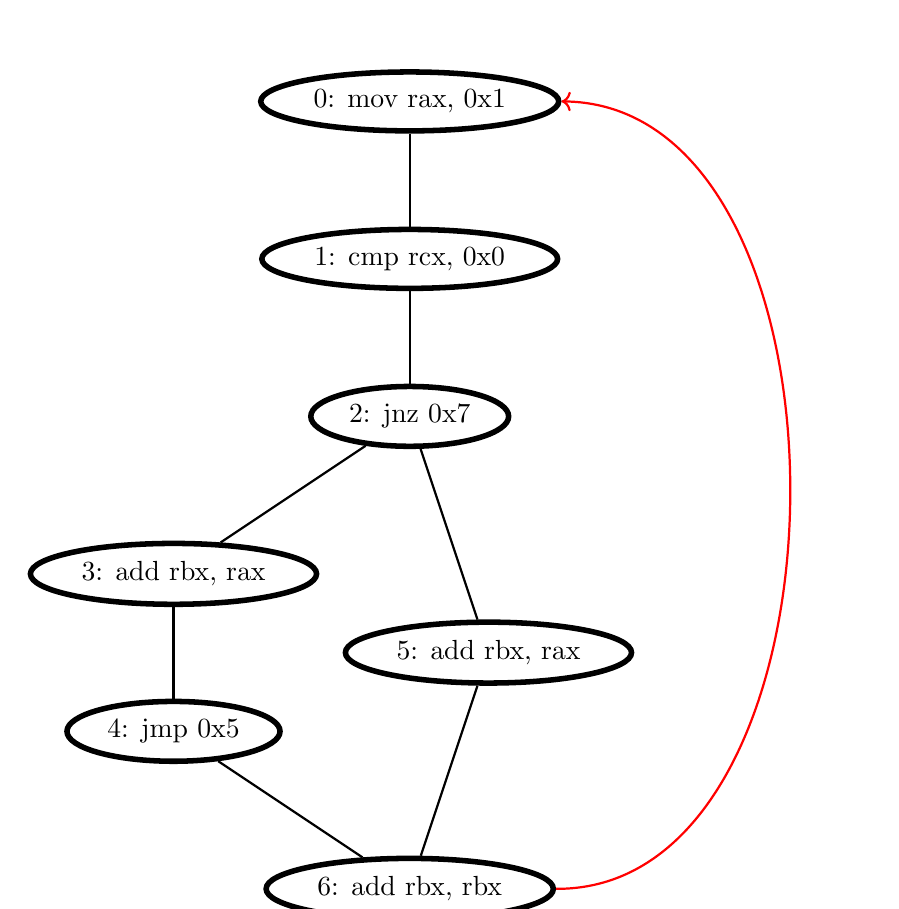
\begin{tikzpicture}
    \node[mynode] (A) at (0, 0)     {0: mov rax, 0x1};	
    \node[mynode] (B) at (0, -2)    {1: cmp rcx, 0x0};
    \node[mynode] (C) at (0, -4)    {2: jnz 0x7};
    \node[mynode] (D) at (-3, -6)   {3: add rbx, rax};
    \node[mynode] (E) at (-3, -8)   {4: jmp 0x5};
    \node[mynode] (F) at (1, -7)    {5: add rbx, rax};
    \node[mynode] (G) at (0, -10)   {6: add rbx, rbx};
    
    
    
    \Edges[](A,B);
    \Edges[](B,C);
    \Edges[](C,D);
    \Edges[](C,F);
    \Edges[](D,E);
    \Edges[](E,G);
    \Edges[](F,G);
    \Edges[style={->, bend right = 90}, color=red](G,A);
    
    \end{tikzpicture}
    \caption{Control flow graph}
    \label{fig:cfg}
\end{figure}

\section{Dependencygraph}
The dependency graph describes all register dependencies that occur in the program. An edge from node $A$ to node $B$ means that the instruction represented by $B$ depends on the instruction represented by $A$. The detailed algorithm that is used to generate this graph can be seen at ~\autoref{sec:depanalysis}.\\
First consider this graph that will be generated in the ``single loop case'' in \autoref{fig:woloop}.\\


\begin{figure}
\centering
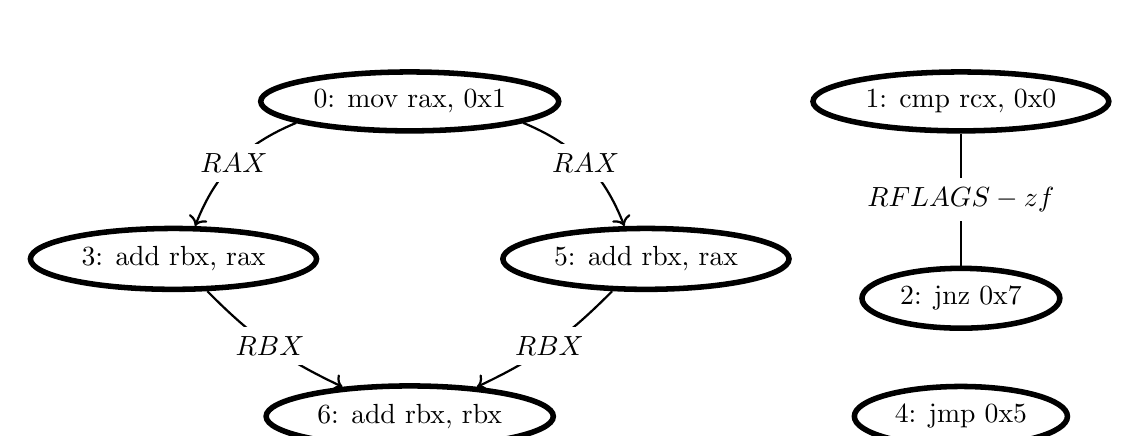
\begin{tikzpicture}
    \node[mynode] (A) at (-4, 0)  {0: mov rax, 0x1};	
    \node[mynode] (B) at (-7, -2) {3: add rbx, rax};
    \node[mynode] (C) at (-1, -2)  {5: add rbx, rax};
    \node[mynode] (D) at (-4, -4) {6: add rbx, rbx};


    \Edges[label=$RAX$, style=bright](A,B);
    \Edges[label=$RAX$, style=bleft](A,C);
    \Edges[label=$RBX$, style={->, bend right = 10}](B,D);
    \Edges[label=$RBX$, style={->, bend left = 10}](C,D);

    \node[mynode] (E)  at (3, 0)  {1: cmp rcx, 0x0};
    \node[mynode] (F)  at (3, -2.5) {2: jnz 0x7};
    
    \Edges[label=$RFLAGS - zf$](E,F);
    
    \node[mynode] (G)  at (3, -4) {4: jmp 0x5};

\end{tikzpicture}
\caption{Dependency graph without loop dependencies}
\label{fig:woloop}
\end{figure}


We can see that this graph was generated with the $CFG$ in mind as there is no edge from node $3$ to node $5$. Additionally we can observe that \suaca\ does differentiate between the different flags contained in the $RFLAGS$ register as the dependence is only reasoned with the $zf$ flag.\\
When \suaca\ is called with at least $2$ loops it will also track all ``loop dependencies''. \autoref{fig:wloop} shows the graph with those in consideration. We can see that two edges were added and they will be colored red to indicate that they were caused by the loops.

\begin{figure}
    \centering
    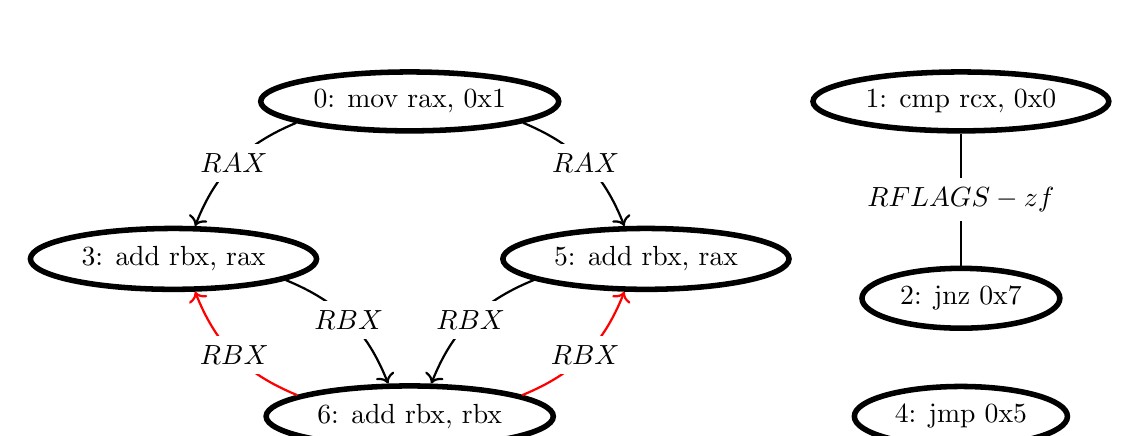
\begin{tikzpicture}
    \node[mynode] (A) at (-4, 0)  {0: mov rax, 0x1};	
    \node[mynode] (B) at (-7, -2) {3: add rbx, rax};
    \node[mynode] (C) at (-1, -2)  {5: add rbx, rax};
    \node[mynode] (D) at (-4, -4) {6: add rbx, rbx};
    
    
    \Edges[label=$RAX$, style=bright](A,B);
    \Edges[label=$RAX$, style=bleft](A,C);
    \Edges[label=$RBX$, style=bleft](B,D);
    \Edges[label=$RBX$, color = red, style=bleft](D, B);
    \Edges[label=$RBX$, style=bright](C,D);
    \Edges[label=$RBX$, color = red, style=bright](D, C);
    
    \node[mynode] (E)  at (3, 0)  {1: cmp rcx, 0x0};
    \node[mynode] (F)  at (3, -2.5) {2: jnz 0x7};
    
    \Edges[label=$RFLAGS - zf$](E,F);
    
    \node[mynode] (G)  at (3, -4) {4: jmp 0x5};
    
    \end{tikzpicture}
    \caption{Dependency graph with loop dependencies}
    \label{fig:wloop}
\end{figure}


\section{Architecture selection}

\section{Detailed information}

\chapter{Algorithms}

When trying to analyze a program the user sometimes needs to fully understand how the results were calculated. Especially if he wants use them to improve his code. Therefore we will discuss \suaca's most important algorithms in the following chapter.

\section{Dependency analysis}
\label{sec:depanalysis}

\subsection{Single iteration}

Here we want to take a look at the algorithm that computes the dependency graph. \\
First we want to discuss a simpler version that ignores the control flow of the program.

\begin{algorithm}[H]
    \SetAlgoLined
    \caption{Dependency analysis without control flow}
    \SetKwInOut{Input}{Input}
    \SetKwInOut{Output}{Output}
    \Input{Instructionlist InstList}
    \Output{Dependencygraph DG}
    Map $:=$ map from Register to line\;
    DG $:=$ Graph that has the same nodes as CFG, but no edges\;
    \ForEach{Instruction $i$ in InstList} {
         \ForEach{Register-Operand $r$ in Operands($i$)} {
             \eIf{IsRead($r$)} {
                 DG.addEdge(Map[$r$], LineOf($i$))\;
             }{
                Map[$r$] = LineOf(i)\;
            }
        }
    }
    \Return DG\;
\end{algorithm}

Where
\begin{itemize}
    \item $Operands(i)$ returns a list of all operands of instruction $i$.
    \item $IsRead(r)$ returns true if the operand $r$ will be read and false if it will be written to.
    \item $LineOf(i)$ returns the line of instruction $i$ in the original program.
\end{itemize}

This algorithm will iterate over all instructions ``line after line''. For each instruction $i$ it will then iterate over all of its operands. For each operand we'll check if it is accessed via read or write. If it is read the algorithm will add an edge from the last written access to the current line. If it is written to the algorithm will map the register to the current line.\\

The runtime of this algorithm can be described as $\mathcal{O}(n*m)$ where $n$ is the number of instructions and $m$ the maximum number of operands that occur in the program.\\

Note that we consider every operand as a register. In practice an operand can of course be a memory address. In this case \suaca\ will extract all registers from that address and treat them as a read operand. \suaca\ will not trace the memory itself.\\

Now we want to take a look at the control flow sensitive algorithm \suaca\ actually uses. 

\begin{algorithm}[H]
    \SetAlgoLined
    \caption{Control flow sensitive dependency analysis}
    \label{alg:dep}
    \SetKwFunction{deps}{Dep-Analysis-Start}
    \SetKwFunction{dep}{Dep-Analysis}
    \SetKwProg{Fn}{Function}{:}{\Return DG\;}
    \Fn{\deps{CFG}}{
        Map $:=$ map from Register to line\;
        DG $:=$ Graph that has the same nodes as CFG, but no edges\;
        Node $:=$ Startnode of CFG\;
        \dep{CFG, DG, Map, Node}\;
    }
    \SetKwProg{Fn}{Function}{:}{}
    \Fn{\dep{CFG, DG, Father-Map, Node}}{
        Map $:=$ copy of Father-Map\;
        \While{HasSuccessor(Node)} {
            \ForEach{Register-Operand $r$ in Operands($i$)} {
                \eIf{IsRead($r$)} {
                    DG.addEdge(Map[$r$], LineOf($i$))\;
                }{
                    Map[$r$] = LineOf(i)\;
                }
            }
            Node $=$ Successor(Node, 0)\;
            \If{numSuccessors(Node) $>$ 1} {
                \dep{CFG, DG, Map, Successor(Node, 1)}\; 
            }
        }
    }
\end{algorithm}

Where
\begin{itemize}
    \item $numSuccessors(Node)$ returns the number of successors of $Node$ in its underlying graph.
    \item $Successor(Node, i)$ returns the $i$th successor of $Node$ in the Graph $Node$ belongs to.
    \item $HasSuccessor(Node)$ returns true if $numSuccessors(Node) >= 1$.
\end{itemize}

This time we'll ``climb along'' the $CFG$. If we never face a branch, i.e.\ $numSuccessors()$ never returns a value greater $1$, this algorithm will exactly the same as the one we have just seen.\\
In the case of $numSuccessors() > 1$ we'll make another call of $Dep-Analysis$ on the ``right branch''. From there on there will be $2$ analyses, one for every branch in the $CFG$. Each analysis has its own $Map$ as there can be different writes on each branch. Note that we won't join the two analyses as we would need to find the first mutual descendant.\\

In the worst case every instruction is a branch, so we would spawn a new function for every one of them. This leads to a runtime of $\mathcal{O}(n^2*m)$.\\

For this algorithm we assume no backbranches, i.e.\ no loops, inside the program. In practice \suaca\ will simply check for every branch if it is a backbranch and should the situation arise ignore it.


\subsection{Multiple iterations}

When telling \suaca\ to run the program in multiple loops we need to adjust the dependency analysis algorithm as there can arise some ``loop dependencies''. To solve this, we'll simply consider the program twice. So we'll append a copy of the program to itself, compute the $CFG$ and then run the algorithm above. Because we know the original length of our program we can extract all ``loop dependencies'' from the resulting dependency graph.

\section{Choosing the ports}
\label{sec:chooseport}

\section{Executing applicable instructions}

\bibliographystyle{alpha}
{\small \bibliography{thesis}}


\end{document}
